\documentclass{article}

\usepackage{booktabs}
\usepackage{tabularx}
\usepackage{graphicx}
\usepackage[table]{xcolor}

\title{Development Plan\\\progname}

\author{\authname}
\setlength\parindent{0pt}
\date{}

%% Comments

\usepackage{color}

\newif\ifcomments\commentstrue %displays comments
%\newif\ifcomments\commentsfalse %so that comments do not display

\ifcomments
\newcommand{\authornote}[3]{\textcolor{#1}{[#3 ---#2]}}
\newcommand{\todo}[1]{\textcolor{red}{[TODO: #1]}}
\else
\newcommand{\authornote}[3]{}
\newcommand{\todo}[1]{}
\fi

\newcommand{\wss}[1]{\authornote{blue}{SS}{#1}} 
\newcommand{\plt}[1]{\authornote{magenta}{TPLT}{#1}} %For explanation of the template
\newcommand{\an}[1]{\authornote{cyan}{Author}{#1}}

%% Common Parts

\newcommand{\progname}{ProgName} % PUT YOUR PROGRAM NAME HERE
\newcommand{\authname}{Team \#, Team Name
\\ Student 1 name and macid
\\ Student 2 name and macid
\\ Student 3 name and macid
\\ Student 4 name and macid} % AUTHOR NAMES                  

\usepackage{hyperref}
    \hypersetup{colorlinks=true, linkcolor=blue, citecolor=blue, filecolor=blue,
                urlcolor=blue, unicode=false}
    \urlstyle{same}
                                


\begin{document}

\begin{table}[hp]
\caption{Revision History} \label{TblRevisionHistory}
\begin{tabularx}{\textwidth}{llX}
\toprule
\textbf{Date} & \textbf{Developer(s)} & \textbf{Change}\\
\midrule
September 26 & N/A & Initial documentation\\
\bottomrule
\end{tabularx}
\end{table}

\newpage

\maketitle

\wss{Put your introductory blurb here.}

\section{Team Meeting Plan}
Weekly meetings are to be held every Saturday at 8:00PM, and additional meetings are to be planned as needed. Any meetings requiring the attendance of team's supervisor will have to be planned based on Dr. Macedo's availability each time. In cases where some team members are absent, each absent team members are expected to bring forward their discussion topics prior to the scheduled meeting time, and review the meeting notes posted in the Discord server. Note-taker is expected to write down meeting notes for each meeting, regardless of the number of participating members.\\

\section{Team Communication Plan}
All main communication channel to be done through team's Discord server, including all meetings. Secondary communication will be through Facebook group chat only if necessary.\\

The following is a screen shot of this team's Discord server:\\
\begin{center}
    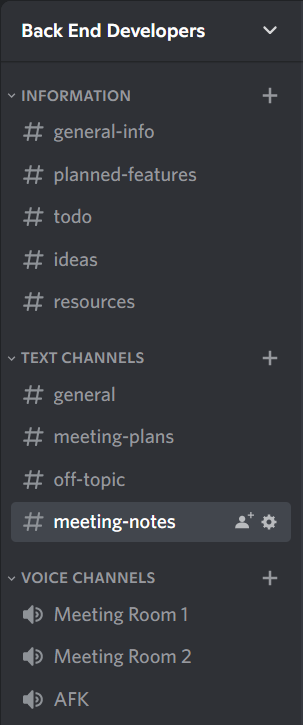
\includegraphics{DiscordServer}
\end{center}

\section{Team Member Roles}

\begin{center}
\begin{tabular}{ | m {3.3cm} | m {3cm} | m{5cm} | }
  \hline
 \cellcolor{black}\color{white}\textbf{Role} & \cellcolor{black}\color{white}\textbf{Name} & \cellcolor{black}\color{white}\textbf{Description}\\ [10pt]
  \hline
 Team Leader & Jonathan Hai \& Jessica Bae & Organize meetings, assign specific tasks to all team members, overlook deliverable deadlines, keep track of overall team project progress, communicate with the TA, the professor, and the supervisor \\
 \hline
 GitHub Leader & Labeeb Zaker \& Nish Shah & Review and approve all Git merge requests from the team  \\  
 \hline
 Meeting Coordinator & Anish Rangarajan & Lead the conversation for team meetings. Responsible for preparing meeting agenda.\\
 \hline
 Note-Taker & Oliver Foote & Take notes during the meeting and post it in the meeting-notes section of Discord channel for record keeping purposes.\\
   \hline
Developer & Everyone & Everyone will work together on the technical component of this project.\\
\hline
\end{tabular}
\end{center}

The task of reviewing rubrics, and each subcomponents of the project will not be assigned to any specific members. These tasks are to be allocated to different members each time, to be decided as needed.\\

\section{Workflow Plan}
Git's branching technique will be used for version control purposes. For any technical commits, everyone is required to put in a formal merge request for GitHub leaders to review and approve or deny. All documentation work does not have to go through GitHub leaders, and can be commited to the main branch right away. Trello will be used for project management purposes (keeping track of non-technical tasks) and Github issue tracker will be used for keeping track of technical tasks.\\

\section{Proof of Concept Demonstration Plan}

The risks for the success of the project lie primarily within the software that is designed. The hardware component in which data is collected will be designed with a relatively simplistic plug-and-play approach in the goal of feeding data to the software component of the project. As many off-the-shelf components and sensors as possible will be used to reduce development overhead and the many possible problems that developing a complex electromechanic system from scratch can involve. However, a proof-of-concept demonstration is still necessary regarding the ergonomics of the project. Should the hardware take on the form of wearable technology (as is currently planned), a demonstration is necessary to show that the system is possible to be worn comfortably, safely, and unintrusively to the user's daily activities.\\

The software system will be the lynchpin of the project. Its goal will be to take the various events that are relevant to Ecological Momentary Assessment (EMA) that the hardware component detects and handle them accordingly. This will involve logging timestamps, locations, environmental factors, and other momentary information, and prompting the user to answer self-survey questions relevant to their current situation. The software system will then process the answers to these questions and momentary data, and will send off the data to the team of physicians handling this person's EMA.\\

Other than the ergonomics, if the hardware component of the system is incapable of sending data and handling output from the software, continuing with the project involves finding a new method of sensing the user's movement, survey answers, and other relevant data and displaying processed information in return. If the software component of the system is incapable of responding to data input from the hardware, processing said data, and returning meaningful results, then the goal of the entire project is rendered moot.\\

The goal for the proof of concept demo will be to demonstrate a functional EMA-enabled software system that can respond to events relevant to EMA, and respond accordingly. This software system will be run locally on a team member's computer. It will be capable of:\\

\begin{itemize}
\item Accepting input in the form of momentary data from events that are triggered as a simulation of real EMA events (such as limps, falls, strange movement patterns, etc.)
\item Prompting the user to answer relevant self-survey questions
\item Displaying information and intaking information from the user simplistically according to common HCI guidelines
\item Processing the inbound EMA and survey data and producing results meaningful to the physicians responsible for the user's EMA
\item Producing graphical representations of said EMA data
\item Sending the processed data and representations to the physicians responsible for the user's EMA
\item Notifying the user about relevant information as a result of processing data (confirmations that data has been sent, recommendations for activity or rest, etc.)
\end{itemize}

Regarding the hardware component of the project, it will be:\\

\begin{itemize}
\item Useable/wearable in a safe, comfortable, and non-intrusive manner optimized for human well-being and overall system performance
\item Placed in a position to collect data relevant to EMA display data regarding EMA related activities
\end{itemize}

\section{Technology}
The following tools shall be used for development in software, embedded systems as well as any support platforms in the system:

\begin{enumerate}
\item Programming languages:
\begin{itemize}
\item Python will be used to generate computer vision code along with several graphical and UI elements. If necessary, Python will also be used for Machine Learning integration.
\item C will be used to program the embedded system (micro-controllers) for efficiency and memory constraints.
\item C\# will be used the team decides to use Unity to create parts of the product.
\item SQL will be used for DBMS and storing data for activity-based tracking.
\end{itemize}
\item Platforms for development:
\begin{itemize}
\item VS code will be used for code-based development.
\item Arduino IDE may be used to code for several existing sensor libraries (gyro meters, Bluetooth modules, Wi-fi modules, etc).
\item STM32Cube IDE for STM32 development. 
\item Autodesk Inventor may be used for creating models for the device and finishing product.
\item MySQL will be used as the platform for interacting with the Database.
\end{itemize}
\item Version control platforms:
\begin{itemize}
\item GitHub will be used for version control for development purposes and general group activity tracking.
\item GitLab will be used for version control (collaborative) with McMaster University.
\end{itemize}
\item Document generation:
\begin{itemize}
\item Latex will be used for generating documentation. TeX distributions that will be used amongst the collaborators are  Texmaker, TeXworks, MikteX and VScode Latex extension.
\end{itemize}
\item Specific plans for Continuous Integration (CI), or an explanation that CI
  is not being done
\begin{itemize}
\item CI will be used to block merge requests until all tests have been passed and approval has been given by atleast two members of the team. 
\item This will speed up development by reducing the overall bugs introduced into the project.
\end{itemize}
\item Measuring tools for code:
\begin{itemize}
\item Coverage.py for measuring code coverage in Python and effectiveness of testing.
\item Valgrind for efficient memory management.
\item Bullseye coverage for C/C++.
\end{itemize}
\item Libraries to use:
\begin{itemize}
\item OpenCV: Open Source computer vision library capable of performing image and video manipulation.
\item Numpy, pandas: Libraries with Python for number and matrix computation/manipulation.
\item HAL libraries: Should we pursue using an ARM architecture chip, the HAL libraries will allow for ease of coding.
\item tkinter: Default python UI library.
\item Several Arduino Sensor libraries to use for interacting with accelerators and other wireless modules.
\end{itemize}
\item Tools to use for project:
\begin{itemize}
\item 3D printer and slicer tools for rapid prototyping.
\item Soldering station and Glue Gun.
\item Wood working tools (Hand Saws and Power Sanding ) if necessary.
\end{itemize}
\end{enumerate}

\section{Coding Standard}
\begin{enumerate}
\item Python:
\begin{itemize} 
\item Code development will closely follow the Google Python Style Guide as a list for do's and don'ts for Python programs.
\item For inline code documentation, Google style doc-strings will be followed for commenting.
\item Pylint will be used as a linter for code development. This linter can be used as an extension to VS code while developing and debugging code.
\end{itemize}
\item C: lint will be used as a linter when programming in C for development and debugging purposes.
\end{enumerate}

\section{Project Scheduling}

\begin{enumerate}
\item Master Project Schedule will be made with a list of all the deadlines, deliverables and Project Implementation tasks. Work will be done based on weekly sprints where tasks will be assigned to each member along with an estimated number of days needed to finish the task. This number is evaluated based on relative complexity of each task.\\

\item Imposed deadline for all tasks are \textbf{two} days before the due date of the deliverable. On this day, the team will conduct a review of all the work done by the members and provide any feedback. The last day before the due date is reserved for making any final changes and small revisions. Moreover, the team will check the completed deliverable with the marking rubric.\\

\item Every two weeks, a design overhaul will be conducted wherein the team will go through the previous parts of the project and update it with any changes made as a result of the current iteration of the project.\\
\end{enumerate}







\end{document}